\documentclass{beamer}
\usepackage[utf8]{inputenc}

\mode<presentation> {
	\usetheme{CambridgeUS}
}
\usepackage{caption}
\captionsetup{font=small,skip=3pt}
\renewcommand{\figurename}{Image}
\usepackage{graphicx}
\usepackage{booktabs}
\usepackage{pgfplots}


\title[Zen architecture]{AMD's Zen microarchitecture}

\author{Jozef Urbanovský} 
\institute[BUT]
{
	Brno University of Technology \\ 
	\medskip
	\textit{xurban66@stud.fit.vutbr.cz}
}
\date{\today}
\begin{document}
	\begin{frame}
		\titlepage
	\end{frame}	
	\begin{frame}
		\frametitle{Overview} 
		\begin{columns}[c] 			
			\column{.5\textwidth} 
			\tableofcontents			
			\column{.3\textwidth}
			\begin{figure}[p]
				\includegraphics[width=\textwidth]{zen.png}
				\caption{Logo}
			\end{figure}			
		\end{columns}
	\end{frame}	
	\section{History}	
	\begin{frame}
		\frametitle{History}
		For years, the only option for mainstream consumers has been Intel CPUs. AMD’s chips lagged 
		far behind, to the point where the only question to be asked about desktop 
		processors was i5 or i7.
		
		With its latest generation of chips based on Zen microarchitecture, called Ryzen, AMD is changing all that. 
		\bigskip
		\begin{itemize}
			\item Development began in August 2012
			\item Introduced at E3 in July 2016
			\item Release planned to be in 2017
			\item First time used with Ryzen 7 series CPUs in February 2017
		\end{itemize}
	\end{frame}	
	%------------------------------------------------
	\section{Features}
	\subsection{Design}	
	\begin{frame}
		\frametitle{Design}
		\begin{columns}[c] 			
			\column{.4\textwidth} 
			\begin{itemize}
				\item L1 write-back cache
				\item 4 ALUs, 2 AGUs/load-store units, and 2 floating-point units per core
				\item SMT (simultaneous multithreading) architecture allows for 2 threads per core
				\item Dedicated stack engine for modifying the stack pointer
			\end{itemize}			
			\column{.53\textwidth}
			\begin{figure}[p]
				\includegraphics[width=\textwidth]{architecture.png}
				\caption{Architecture}
			\end{figure}			
		\end{columns}
	\end{frame}	
	%------------------------------------------------
	\subsection{Advantages over predecessors}	
	\begin{frame}
		\frametitle{Advantages over predecessors}
		\begin{block}{Manufacturing process}
			\begin{itemize}
				\item 14 nm FinFET silicon
				\item Metal-insulator-metal process to increase the clock speeds and reduce voltages
			\end{itemize}
		\end{block}		
		\begin{block}{Performance}
			\begin{itemize}
				\item 52\% improvement in IPC over its predecessor 
				\item Dynamic scaleability of frequence and voltage
				\item Each core processes up to two threads
			\end{itemize}
		\end{block}		
		\begin{block}{Memory}
			\begin{itemize}
				\item 3D-stacked DRAM - High Bandwidth Memory 
				\item Up to 8 channels of DDR4 memory	
			\end{itemize}
		\end{block}
	\end{frame}	
	%------------------------------------------------
	\section{Products}
	\subsection{Ryzen}	
	\begin{frame}
		\frametitle{Summit Ridge}
		\begin{columns}[c]			
			\column{.45\textwidth} 
			\textbf{Specifications}
			\begin{itemize}
				\item AM4 socket
				\item 4.8 billion transistors on 8-core design
				\item 192 mm$^2$ die size
				\item Supports up to DDR4-3600
				\item Supports x87, MMX, SSE
			\end{itemize}			
			\column{.5\textwidth}
			\textbf{Codename:}
			Summit Ridge \bigskip
						
			Ryzen is an AMD brand for microprocessors implementing their Zen microarchitecture.
			
			CPUs feature unlocked multipliers across the board for overclocking.			
		\end{columns}
	\end{frame}	
	%------------------------------------------------
	\begin{frame}
		\frametitle{Ryzen CPUs}
		\begin{table}			
			\begin{tabular}{l c c c c}
				\toprule
				\textbf{Model} & \textbf{Cores/Threads} & \textbf{Clock speeds} & \textbf{L3 Cache} & \textbf{TDP}\\
				\midrule
				7 1800X & 8/16 & 3.6 - 4.0 [GHz] & 16 MB & 95 W\\
				7 1700 & 8/16 & 3.0 - 3.7 [GHz] & 16 MB & 65 W\\
				5 1600X & 6/12 & 3.6 - 4.0 [GHz] & 16 MB & 95 W\\
				5 1500X & 4/8 & 3.5 - 3.7 [GHz] & 8 MB & 65 W\\
				\bottomrule
			\end{tabular}
			\caption{Specifications of unveiled CPUs}
		\end{table}	
		\begin{figure}[p]
			\includegraphics[width=.4\textwidth]{ryzen.png}
			\caption{Ryzen CPU}
		\end{figure}
	\end{frame}	
	%------------------------------------------------
	\section{Benchmarks}
	%------------------------------------------------	
	\begin{frame}
		\frametitle{Benchmarks}
		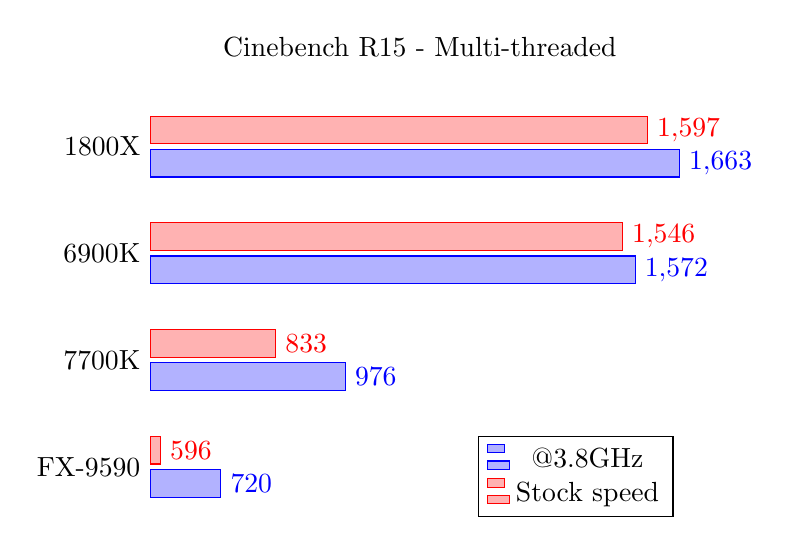
\begin{tikzpicture}
		\begin{axis}[title  = Cinebench R15 - Multi-threaded,
		xbar,
		y axis line style = { opacity = 0 },
		axis x line       = none,
		tickwidth         = 0pt,
		enlarge y limits  = 0.2,
		enlarge x limits  = 0.02,
		symbolic y coords = {FX-9590, 7700K, 6900K, 1800X},
		nodes near coords,
		legend pos=south east,
		]
		\addplot coordinates { (1663,1800X) (976,7700K) (1572,6900K) (720,FX-9590) };
		\addplot coordinates { (1597,1800X) (833,7700K) (1546,6900K) (596,FX-9590) };
		\legend{@3.8GHz, Stock speed}
		\end{axis}
		\end{tikzpicture}
		\begin{center}
			\footnotesize{Cinebench score (higher is better)}
		\end{center}		
	\end{frame}	
	%------------------------------------------------
	\section{Conclusion}
	\begin{frame}
		\frametitle{Conclusion}
		\begin{center}
		The march towards Ryzen has been a long road for AMD. Anyone creating a new CPU
		microarchitecture deserves credit as designing such a complex thing requires millions 
		of hours of hard graft. AMD’s targets of low power, small area, and high-performance 
		while using x86 instructions was a spectacularly high bar, but they delivered. 
		\end{center}
		\begin{figure}[p]
			\includegraphics[width=.5\textwidth]{die.jpg}
			\caption{Die shot of Ryzen 7 1800X}
		\end{figure}
	\end{frame}	
	%------------------------------------------------	
	\begin{frame}
		\frametitle{Citation}
		\begin{center}
			"Time for Ryzen has arrived." - Lisa T. Su
		\end{center}
	\end{frame}
	%------------------------------------------------
	\begin{frame}
		\frametitle{References}
		\footnotesize{
			\begin{thebibliography}{99}	
				\bibitem[Wikipedia, 2017]{p1} Zen (microarchitecture)
				\newblock \url{https://en.wikipedia.org/wiki/Zen_(microarchitecture)}
				\bibitem[Wikipedia, 2017]{p2} Ryzen
				\newblock \url{https://en.wikipedia.org/wiki/Ryzen}
				\bibitem[AMD Ryzen, 2017]{p3} AMD Ryzen
				\newblock \url{https://www.amd.com/en/ryzen}
				\bibitem[Tom's Hardware, 2017]{p4} Tom's Hardware Ryzen 7 1800X review
				\newblock \url{http://www.tomshardware.com/reviews/amd-ryzen-7-1800x-cpu,4951.html}
				\bibitem[Anandtech, 2017]{p3} The AMD Zen and Ryzen 7 Review: A Deep Dive on 1800X, 1700X and 1700
				\newblock \url{http://www.anandtech.com/show/11170/the-amd-zen-and-ryzen-7-review-a-deep-dive-on-1800x-1700x-and-1700/23}
			\end{thebibliography}
		}
	\end{frame}
	%------------------------------------------------
	\begin{frame}
		\begin{figure}[p]
			\centering
			\includegraphics[width=0.5\textwidth]{thanks.png}
		\end{figure}
	\end{frame}
	%----------------------------------------------------------------------------------------
\end{document} 